%
%--- 
%-----------------------------------
\chapter{Monte Carlo simulation}
\label{ch:Monte-Carlo-simulation}
%-----------------------------------
%--- 
%

In order to predict experimental quantities in nMOTs, we propose a Monte Carlo simulation to estimate the probability distributions of both the atoms' position and velocity. The goal is to acquire simulated quantities in agreement with experimental measures for different nMOTs by considering as many parameters as possible. Our simulation can be used to optimize the parameters of nMOTs without the necessity of experimental data. It is also a tool to analyse the feasibility of unusual nMOT arrangements such as nMOTs with fewer laser beams. To ensure optimization, we developed a module for Python using the C programming language\footnote{We choose the C language since it is one of the fastest languages available.}, which deploys our model. We also developed a Python program that applies the model-view-controller pattern and parallelism. Our code is available in \cite{nMOT_sim}. In this section, we shall introduce our model as well as its deployment.

% Stochastic evolution
%-----------------------------------
%
%-----------------------------------
\section{Stochastic evolution}
\label{sec:stochastic-evolution}
%-----------------------------------
%

Let us consider an atom at $ \mathbf{r_0} $ and with the velocity $ \mathbf{v_0} $ in the presence of laser beams and a quadrupole magnetic field. After a period $ \delta t $, this atom can absorb a photon with momentum $ \hbar \mathbf{k_j} $ and then emit a photon with momentum $ \hbar |\mathbf{k}_j| \mathbf{\hat{u}} $, where $ \mathbf{\hat{u}} $ is an uniform unit random vector and $ \mathbf{k}_j $ is the wave vector of the $j$-th laser beam. Also, since there is a magnetic field gradient, a magnetic force acts on the atom as discussed in section \ref{sec:magnetic-force} that yields a position-dependent acceleration $ \mathbf{a}_{B}(\mathbf{r_0}) $. Therefore, the atom's velocity $ \mathbf{v}_i $ and position $ \mathbf{r}_i $ at instant $ i \delta t $, where $ i = 0, 1, \cdots $, are
\begin{equation}
    \mathbf{v}_{i} = \left\{ \begin{array}{lr}
        \mathbf{v}_{i - 1} + \hbar \frac{|\mathbf{k}_j|}{m}(\mathbf{\hat{k}}_j + \mathbf{\hat{u}}) + (\mathbf{a}_B(\mathbf{r}_{i - 1})- g \mathbf{\hat{z}}) \delta t, & \textrm{with probability}\ P_{i,j}
        \\
        \mathbf{v}_{i - 1} + (\mathbf{a}_B(\mathbf{r}_{i - 1})- g \mathbf{\hat{z}}) \delta t, & \textrm{with probability}\ 1 - \sum_{j} P_{i,j}
        \end{array} \right.
        \label{eq:atom-velocity-iteration}
\end{equation}
and
\begin{equation}
    \mathbf{r}_i = \mathbf{r}_{i - 1} + \mathbf{v}_{i}\delta t + (\mathbf{a}_B(\mathbf{r}_{i - 1}) - g \mathbf{\hat{z}}) \delta t^2 / 2,
    \label{eq:atom-position-iteration}
\end{equation}
where $ P_{i,j} $ is the probability of happing a scattering event due to the $ j $-th laser beam also known as \textbf{transition probability}. Since $ P_{i,j} $ is a conditional probability that depends only on the previous atom state, the dynamics is then a \textbf{memoryless stochastic process}, also known as \textbf{Markov chain}. The goal is to sample trajectories $ \mathbf{r}(t) $ and velocities $ \mathbf{v}(t) $ in order to estimate the probability distributions of the atom's position and velocity. To perform this, we iterate the equations (\ref{eq:atom-velocity-iteration}) and (\ref{eq:atom-position-iteration}) and then fill up histograms.


%-----------------------------------
\subsection{Equilibrium}
\label{sec:equilibrium}
%-----------------------------------

Let us consider the vector $ \rho(t) = \rho(i\delta) = \rho_i $ in which each component is the probability of an atom being at specific position $ \mathbf{r} = (x, y, z) $ with a specific velocity $ \mathbf{v} = (v_x, v_y, v_z) $ at a instant $ t $.
We shall call this vector as \textbf{atom state}. Although position and velocity are continuous variables, we must discrete both to perform a feasible computation. If we consider $ N $ possible values for $ x $, $ y $, $ z $, $ v_x $, $ v_y $, and $ v_z $, the dimension of the vector $ \rho_i $ is $ N^6 $, which means that the dimension of the problem escalates very quickly. Since the probabilities related to each component of position ($ x $, $ y $, and $ z $) and velocity ($ v_x $, $ v_y $, and $ v_z $) are independent, we only need the marginal distributions so that the total dimension will be reduced to $ 6N $. It is also possible to represent the transition probabilities $ P_i $ in the same vector space as a matrix $ \mathbf{P} $ of which each element is $ P_{i,j} $\footnote{We are assuming that $ \mathbf{r} $ and $ \mathbf{v} $ are discrete variables}. Therefore, after $ n $ iterations, the atom state will be \cite[Section~23.2]{wasserman2004all}
\begin{equation}
    \rho_n =  \rho_0 \underbrace{(\mathbf{P} \times \mathbf{P} \times \cdots \times \mathbf{P})}_{\textrm{mutiply the matrix $n$ times}} = \rho_0 \mathbf{P}^n,
\end{equation}
where $ \rho_0 $ is the initial atom state given by a deterministic vector since we set the initial atom's position and velocity. We expect that $ \rho $ be constant after a sufficient number of iterations, which it is observed experimentally. Thus, $ \rho = \rho\mathbf{P} $ for large enough $ n $. In this case, we say that $ \rho $ is \textbf{stationary}. The purpose of the simulation is to estimate the atom state $ \rho $. In order to obtain proper samples of $ \rho $, we only save $ \mathbf{r} $ and $ \mathbf{v} $ after a number of iterations.

%-----------------------------------
\subsection{Magnetic field basis}
\label{sec:magnetic-field-basis}
%-----------------------------------

\begin{wrapfigure}{l}{0.4\textwidth}
    \centering
    \vspace{-10px}
    \caption{Magnetic field basis}
    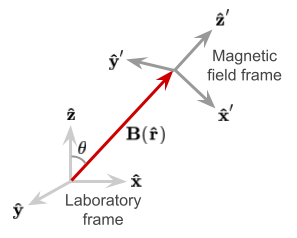
\includegraphics[width=0.3\textwidth]{USPSC-img/polarization_basis.png}
    \legend{basis $ A' = \{\mathbf{\hat{x}}', \mathbf{\hat{y}}', \mathbf{\hat{z}}'\} $ of the magnetic field frame in relation to the basis $ A = \{\mathbf{\hat{x}}, \mathbf{\hat{y}}, \mathbf{\hat{z}}\} $ of the laboratory frame. \\ Source: author}
    \label{fig:magnetic-field-basis}
    \vspace{0px}
\end{wrapfigure}

We shall consider the assumptions introduced in section \ref{sec:MOT-force}, which simplifies a four-level system in three independent two-level systems associated with the polarizations $ \sigma_{\pm} $ and $ \pi $. In this condition, for each laser beam, there are three possible transitions, each one with its scattering rate $ R_{i,j,l} $, where $ l \in \{\sigma_{+}, \sigma_{-}, \pi \} $. Initially, we define the laser polarizations on the basis $ \mathbf{B} = \{\hat{\sigma}_{+}, \hat{\sigma}_{-}, \hat{\pi} \} $ so that
\begin{equation}
    \hat{\sigma}_+ = \frac{\mathbf{\hat{x}} + i\mathbf{\hat{y}}}{\sqrt{2}},\ \ \hat{\sigma}_- = \frac{\mathbf{\hat{x}} - i\mathbf{\hat{y}}}{\sqrt{2}},\ \ \hat{\pi} = \mathbf{\hat{z}},
\end{equation}
where $ A = \{\mathbf{\hat{x}}, \mathbf{\hat{y}}, \mathbf{\hat{z}}\} $ is the basis of the laboratory frame. To account the magnetic field $ \mathbf{B} $ effect in $ R_{i,j,l} $, we must analyse the magnetic field in a frame that defines the quantization axis parallel to $ \mathbf{B} $. Let us consider the basis $ A' = \{\mathbf{\hat{x}}', \mathbf{\hat{y}}', \mathbf{\hat{z}}'\} $ in the the magnetic field frame as illustrated in figure \ref{fig:magnetic-field-basis}.

The polarization basis $ \mathbf{B}' = \{\hat{\sigma}_{+}', \hat{\sigma}_{-}', \hat{\pi}' \} $ in the magnetic field frame is given by
\begin{equation}
    \hat{\sigma}_+' = \frac{\mathbf{\hat{x}'} + i\mathbf{\hat{y}}'}{\sqrt{2}},\ \ \hat{\sigma}_-' = \frac{\mathbf{\hat{x}'} - i\mathbf{\hat{y}}'}{\sqrt{2}},\ \ \hat{\pi}' = \mathbf{\hat{z}}' \| \mathbf{B}.
\end{equation}

Let us consider the polarization vector $ \hat{\epsilon}_j $ of the $ j $-th laser beam defined as $ [\hat{\epsilon}_j]_B $ on the laboratory basis $ B $. Its components on the basis $ B' $ is given by $ [\hat{\epsilon}_j]_B' = M [\hat{\epsilon}_j]_B $, where $ M $ is the change-of-basis matrix. We must consider two other change-of-basis matrices to obtain $ M $. The first one is the matrix $ M' $ that change a polarization basis such as $ B $ to a Cartesian basis such as $ A $. The second one is the rotation matrix $ R(\theta) $. Thus, the change-of-basis $ M $ is given by
\begin{equation}
    M = (M')^{\dagger}R(\theta)M',\ \ (M')^{\dagger} = ((M')^*)^T = (M')^{-1},
\end{equation}
where
\begin{equation}
    M' = \left[ \begin{matrix}
        1/\sqrt{2} & 1/\sqrt{2} & 0 \\
        -i/\sqrt{2} & i/\sqrt{2} & 0 \\
        0 & 0 & 1
    \end{matrix} \right],\ \
    R(\theta) = \left[ \begin{matrix}
        1 & 0 & 0 \\
        0 & \cos(\theta) & -\sin(\theta) \\
        0 & \sin(\theta) & \cos(\theta)
    \end{matrix} \right].
\end{equation}

%-----------------------------------
\subsection{Transition probabilities}
\label{sec:transition-probabilities}
%-----------------------------------

The scattering rate $ R_{i,j,l} $ is essentially the time derivative of the probability of scattering a photon of the $j$-th laser beam due to transition $ l $. Hence, the probability $ P_{i,j,l} $ of happing a scattering event during a time interval $ \delta t $ is given by
\begin{equation}
    R_{i,j,l} = \frac{\partial P_{i,j,l}}{\partial t} \Rightarrow P_{i,j,l} \simeq R_{i,j,l} \delta t.
\end{equation}
The probability of a photon from the $j$-th laser beam having the polarization $ l $ is $ \left| \braket{\hat{\epsilon}_j|\mathbf{\hat{e}}_l} \right| $, where $ \mathbf{\hat{e}}_l \in B' $. Thus, the transition probability $ P_{i,j} $ is given by
\begin{equation}
    P_{i,j} = \sum_{l} \left| \braket{\hat{\epsilon}_j|\mathbf{\hat{e}}_l} \right| P_{i,j,k} =  \sum_{l} \left| \braket{\hat{\epsilon}_j|\mathbf{\hat{e}}_l} \right| R_{i,j,l} \delta t.
\end{equation}
From equation (\ref{eq:radiation-pressure-force-2}), we have
\begin{equation}
    R_{i,j,l} = \frac{\Gamma}{2}\frac{s(\mathbf{r})}{1 + s(\mathbf{r}) + (2\Delta_l / \Gamma)^2},\ \ s(\mathbf{r}) = \exp\left[\ -\frac{2(x^2 + y^2)}{w^2} \right],\ \ \Delta_l = \delta + \delta_Z^{(l)} + \delta_D,
\end{equation}
where $ w $ is the waist of the $ j $-th laser beam, $ \delta $ is the laser detuning, $ \delta_Z^{(l)} $ is the Zeeman shift due to the $ l $ transition given by equation (\ref{eq:Zeeman-shift}), and $ \delta_D = - \mathbf{k} \cdot \mathbf{v}_{i - 1} $ is the Doppler shift. To increase accuracy, we are taking into account the Gaussian profile of the laser beams in $ s(\mathbf{r}) $.

%-----------------------------------
%

% Monte Carlo Simulation
%-----------------------------------
%
%-----------------------------------
\section{Input and outputs}
\label{sec:input-outputs}
%-----------------------------------
%

Overall, the input of the simulation is divided into two categories: the \textbf{experiment} and the \textbf{performance parameters}. The experiment parameters include information about the controllable quantities of a nMOT, such as the laser arrangement, the magnetic field profile, and the involved electronic transitions. It is essential to have detailed information about the nMOT in order to accurately obtain experimental quantities. The performance parameters define precision, execution time, and memory usage. We seek the optimisation of both time and spatial computational complexities. Hence, it is important to properly set up the performance parameters in order to execute a simulation in an acceptable period of time using the available memory.

The raw output of the simulation is six probability distributions of the atoms' position and velocity, as explained in Section \ref{sec:equilibrium}. The position distributions are essential to obtaining experimental quantities related to the atomic cloud profile, such as the centre of mass and the cloud size. While the velocity distributions are relevant to obtaining the temperature.

%-----------------------------------
\subsection{Input}
\label{sec:input}
%-----------------------------------

The \textbf{experiment parameters} are presented in three groups: the laser arrangement, the magnetic field profile, and the involved electronic transition. All groups are shown in tables \ref{tab:transition-parameters}, \ref{tab:magnetic-field-profile-parameters}, and \ref{tab:laser-beams-arrangement-parameters}. Table \ref{tab:transition-parameters} contains essential information to define the involved electronic transition as well as the atoms' mass, which is crucial for evaluating the scattering rates (\ref{eq:scattering-rate-each-transition}) and therefore the transition probabilities (\ref{eq:transition-probabilities}).
Table \ref{tab:magnetic-field-profile-parameters} contains the magnetic field profile. Besides the quadrupole magnetic field already mentioned in previous sections, some experiments also have a residual linear gradient and a constant magnetic field to control the magnetic field origin. Lastly, table \ref{tab:laser-beams-arrangement-parameters} defines the laser beam arrangement.

\begin{table}[ht!]
    \centering
    \begin{tabular}{|c|c|c|}
        \hline
        \textbf{Symbol} & \textbf{Description} & \textbf{Unit} \\ \hline
        $ \Gamma $ & Natural linewidth & $ 2\pi \times kHz $ \\
        $ \lambda $ & Resonance wavelength & $ nm $ \\
        $ J_{\textrm{gnd}} $ & Total angular momentum of the ground state & dimensionless \\
        $ J_{\textrm{exc}} $ & Total angular momentum of the excited state & dimensionless \\
        $ g_{\textrm{gnd}} $ & \textit{Landé} factor of the ground state & dimensionless \\
        $ g_{\textrm{exc}} $ & \textit{Landé} factor of the excited state & dimensionless \\
        $ m $ & Atomic mass & $ Da $ (Dalton unit) \\
        \hline
    \end{tabular}
    \caption{Parameters that defines the involved electronic transition and the mass of the atoms.}
    \label{tab:transition-parameters}
\end{table}

\begin{table}[ht!]
    \centering
    \begin{tabular}{|c|c|c|}
        \hline
        \textbf{Symbol} & \textbf{Description} & \textbf{Unit} \\ \hline
        $ B_0 $ & Magnetic field gradient in equation (\ref{eq:magnetic-field-profile}) & $ G/cm $ \\
        $ B_{\textrm{axial}} $ & Axial direction of the magnetic field & 3D vector \\
        $ B_{\textrm{lingrad}} $ & Residual magnetic field gradient & 3D vector \\
        $ B_{\textrm{bias}} $ & Constant magnetic field & 3D vector \\
        \hline
    \end{tabular}
    \caption{Parameters that defines the magnetic field profile.}
    \label{tab:magnetic-field-profile-parameters}
\end{table}

\begin{table}[ht!]
    \centering
    \begin{tabular}{|c|c|c|}
        \hline
        \textbf{Symbol} & \textbf{Description} & \textbf{Unit} \\ \hline
        $ \delta $ & Laser detuning & $ 2\pi \times kHz $ \\
        $ s_0 $ & Saturation parameter & dimensionless \\
        $ w $ & Waist & $ cm $ \\
        $ \hat{\mathbf{k}} $ & Wavevector direction & 3D vector \\
        $ \hat{\epsilon} $ & Polarization vector in the laboratory frame & 3D vector \\
        \hline
    \end{tabular}
    \caption{Parameters that defines the laser beams arrangement.}
    \label{tab:laser-beams-arrangement-parameters}
\end{table}

The \textbf{performance parameters} are shown in table \ref{tab:performance-parameters}. Let us discussed each of them. The parameter $ t_{w} $ is the period of time in which we do not get samples. This parameter defines a moment at which equilibrium has already been reached. We set its value by analysing the variation of the atom's position. Thus, we only get samples during the interval $ t - t_{w} $. The last time parameter is the time resolution from equations (\ref{eq:atom-velocity-iteration}) and (\ref{eq:atom-position-iteration}). The parameters $ t $, $ r_{m} $, and $ v_{m} $ define the conditions to stop the simulation, which are
\begin{itemize}
    \item If the simulation time is greater than $ t $;
    \item If the atom trespasses the sphere of radius $ r_{m} $;
    \item If the atom's velocity is greater than $ v_{m} $.
\end{itemize}
The position and velocity resolution are defined by the parameters $ N_{r} $, $ r_{m} $, $ v_{m} $. The spatial resolution is $ \delta r = r_{m} / N_{r} $, whilst the speed resolution is $ \delta v = v_{m} / N_r $. Hence, the atoms' positions $ x $, $ y $, and $ z $ are multiples of $ \delta_r $, whereas the atoms' velocities $ v_x $, $ v_y $, and $ v_z $ are multiples of $ \delta_v $. The number of samples $ N_{s} $ is basically the number of ensembles (atoms' motions), which defines the precision of the output. Lastly, the initial temperature $ T_0 $ defines the initial atoms' velocities by sampling the \textbf{Maxwell-Boltzmann distribution}.

\begin{table}[ht!]
    \centering
    \begin{tabular}{|c|c|c|}
        \hline
        \textbf{Symbol} & \textbf{Description} & \textbf{Unit} \\ \hline
        $ t $ & Maximum time of simulation & $ ms $ \\
        $ t_{w} $ & Waiting time & $ ms $ \\
        $ \delta t $ & Time resolution & $ ms $ \\
        $ r_{m} $ & Maximum distance of the origin & $ cm $ \\
        $ v_{m} $ & Maximum speed & $ cm / s $ \\
        $ N_{s} $ & Number of samples & dimensionless \\
        $ N_{r} $ & Resolution number & dimensionless \\
        $ N_{p} $ & Number of parallel tasks & dimensionless \\
        $ T_0 $ & Initial temperature & $ \mu K $ \\
        \hline
    \end{tabular}
    \caption{Performance parameters.}
    \label{tab:performance-parameters}
\end{table}

%-----------------------------------
\subsection{Output}
\label{sec:output}
%-----------------------------------

The raw output of the simulation consists of six probability distributions that describe the atoms' motion. These distributions can be divided into two groups: \textbf{position} and \textbf{velocity distributions}. Although these are continuous quantities, our model reproduces discrete values. Hence, the atoms' position and velocities are then restricted to the following space
\begin{gather}
    \mathbf{r} = (i_x \hat{\mathbf{x}} + i_y \hat{\mathbf{y}} + i_z \hat{\mathbf{z}}) \delta r, \\
    \mathbf{v} = (j_x \hat{\mathbf{x}} + j_y \hat{\mathbf{y}} + j_x \hat{\mathbf{z}}) \delta v,
\end{gather}
where $ i_x $, $ i_y $, $ i_z $, $ j_x $, $ j_y $, and $ j_z $ are positive integers, and $ \delta r $ and $ \delta v $ are the spatial and speed resolution respectively. The joint probability distribution $d_r$ of the atoms' position is given by
\begin{gather}
    d_{r}(i_x, i_y, i_z) = d_x(i_x) d_y(i_y) d_z(i_z),
    \label{eq:joint-position-distribution}
    \\
    \sum_{V} d_r(i_x,i_y,i_z) \ \rightarrow\ \textrm{Probability of finding an atom in the volume $ V $},
\end{gather}
where $ d_{x} $, $ d_y $, and $ d_z $ are marginal probability distributions. The equation (\ref{eq:joint-position-distribution}) assumes independence between each direction. Similarly, the joint probability distribution $d_v$ of the atoms' velocity is given by
\begin{gather}
    d_{v}(i_{v_x}, i_{v_y}, i_{v_z}) = d_{v_x}(i_{v_x}) d_{v_y}(i_{v_y}) d_{v_z}(i_{v_z}),
    \label{eq:joint-velocity-distribution}
    \\
    \sum_{\Delta v} d_{v}(i_{v_x}, i_{v_y}, i_{v_z}) \ \rightarrow\ \textrm{Probability of finding an atom with velocities $ \Delta v $},
\end{gather}

We are interested in two atomic cloud quantities: the centre of mass and the cloud size. The centre of mass is given by,
\begin{equation}
    \mathbf{r}_c = \braket{d_x} \hat{\mathbf{x}} + \braket{d_y} \hat{\mathbf{y}} + \braket{d_z} \hat{\mathbf{z}},
    \label{eq:simulated-centre-of-mass}
\end{equation}
where $ \braket{d_x} $, $ \braket{d_y} $, and $ \braket{d_z} $ are averages. The cloud sizes are
\begin{equation}
    \sigma_x = \sqrt{\braket{(d_x - \braket{d_x})^2}},\ \sigma_y = \sqrt{\braket{(d_y - \braket{d_y})^2}},\ \sigma_z = \sqrt{\braket{(d_z - \braket{d_z})^2}},
    \label{eq:simulated-cloud-sizes}
\end{equation}
where $ \sigma_x $, $ \sigma_y $, $ \sigma_z $ are standard deviations.

We are also interested in temperature, which is evaluated by the equipartition theorem given by
\begin{equation}
    \frac{3}{2}k_B T = \frac{m}{2} (\braket{d_{v_x}^2} + \braket{d_{v_y}^2} + \braket{d_{v_z}^2})\ \Rightarrow\ T = \frac{m}{3k_B} (\braket{d_{v_x}^2} + \braket{d_{v_y}^2} + \braket{d_{v_z}^2}).
\end{equation}

%-----------------------------------
%
